\documentclass[12pt]{article}
\usepackage{amsmath}
\usepackage{amssymb}
\usepackage[letterpaper,top=1in,bottom=1in,left=0.75in,right=0.75in,centering]{geometry}
%\usepackage{fancyhdr}
\usepackage{enumerate}
%\usepackage{lastpage}
\usepackage{multicol}
\usepackage{graphicx}
\usepackage{hyperref}

\reversemarginpar

%\pagestyle{fancy}
%\cfoot{}
%\lhead{Math 1560}\chead{Test \# 1}\rhead{May 18th, 2017}
%\rfoot{Total: 10 points}
%\chead{{\bf Name:}}
\newcommand{\points}[1]{\marginpar{\hspace{24pt}[#1]}}
\newcommand{\skipline}{\vspace{12pt}}
%\renewcommand{\headrulewidth}{0in}
\headheight 30pt

\newcommand{\di}{\displaystyle}
\newcommand{\abs}[1]{\lvert #1\rvert}
\newcommand{\len}[1]{\lVert #1\rVert}
\renewcommand{\i}{\mathbf{i}}
\renewcommand{\j}{\mathbf{j}}
\renewcommand{\k}{\mathbf{k}}
\newcommand{\R}{\mathbb{R}}
\newcommand{\aaa}{\mathbf{a}}
\newcommand{\bbb}{\mathbf{b}}
\newcommand{\ccc}{\mathbf{c}}
\newcommand{\dotp}{\boldsymbol{\cdot}}
\newcommand{\bbm}{\begin{bmatrix}}
\newcommand{\ebm}{\end{bmatrix}}                   
                  
\begin{document}


\author{Instructor: Sean Fitzpatrick}
\thispagestyle{empty}
\vglue1cm
\begin{center}
{\bf MATH 2565 - Tutorial \#12 Solutions}
\end{center}




%\thispagestyle{empty}



\textbf{Assigned problems}

 \begin{enumerate}
\item Plot the given polar function:

\begin{enumerate}
\item $r=\cos(2\theta)$, $\theta\in [0,2\pi]$.


\begin{center}
 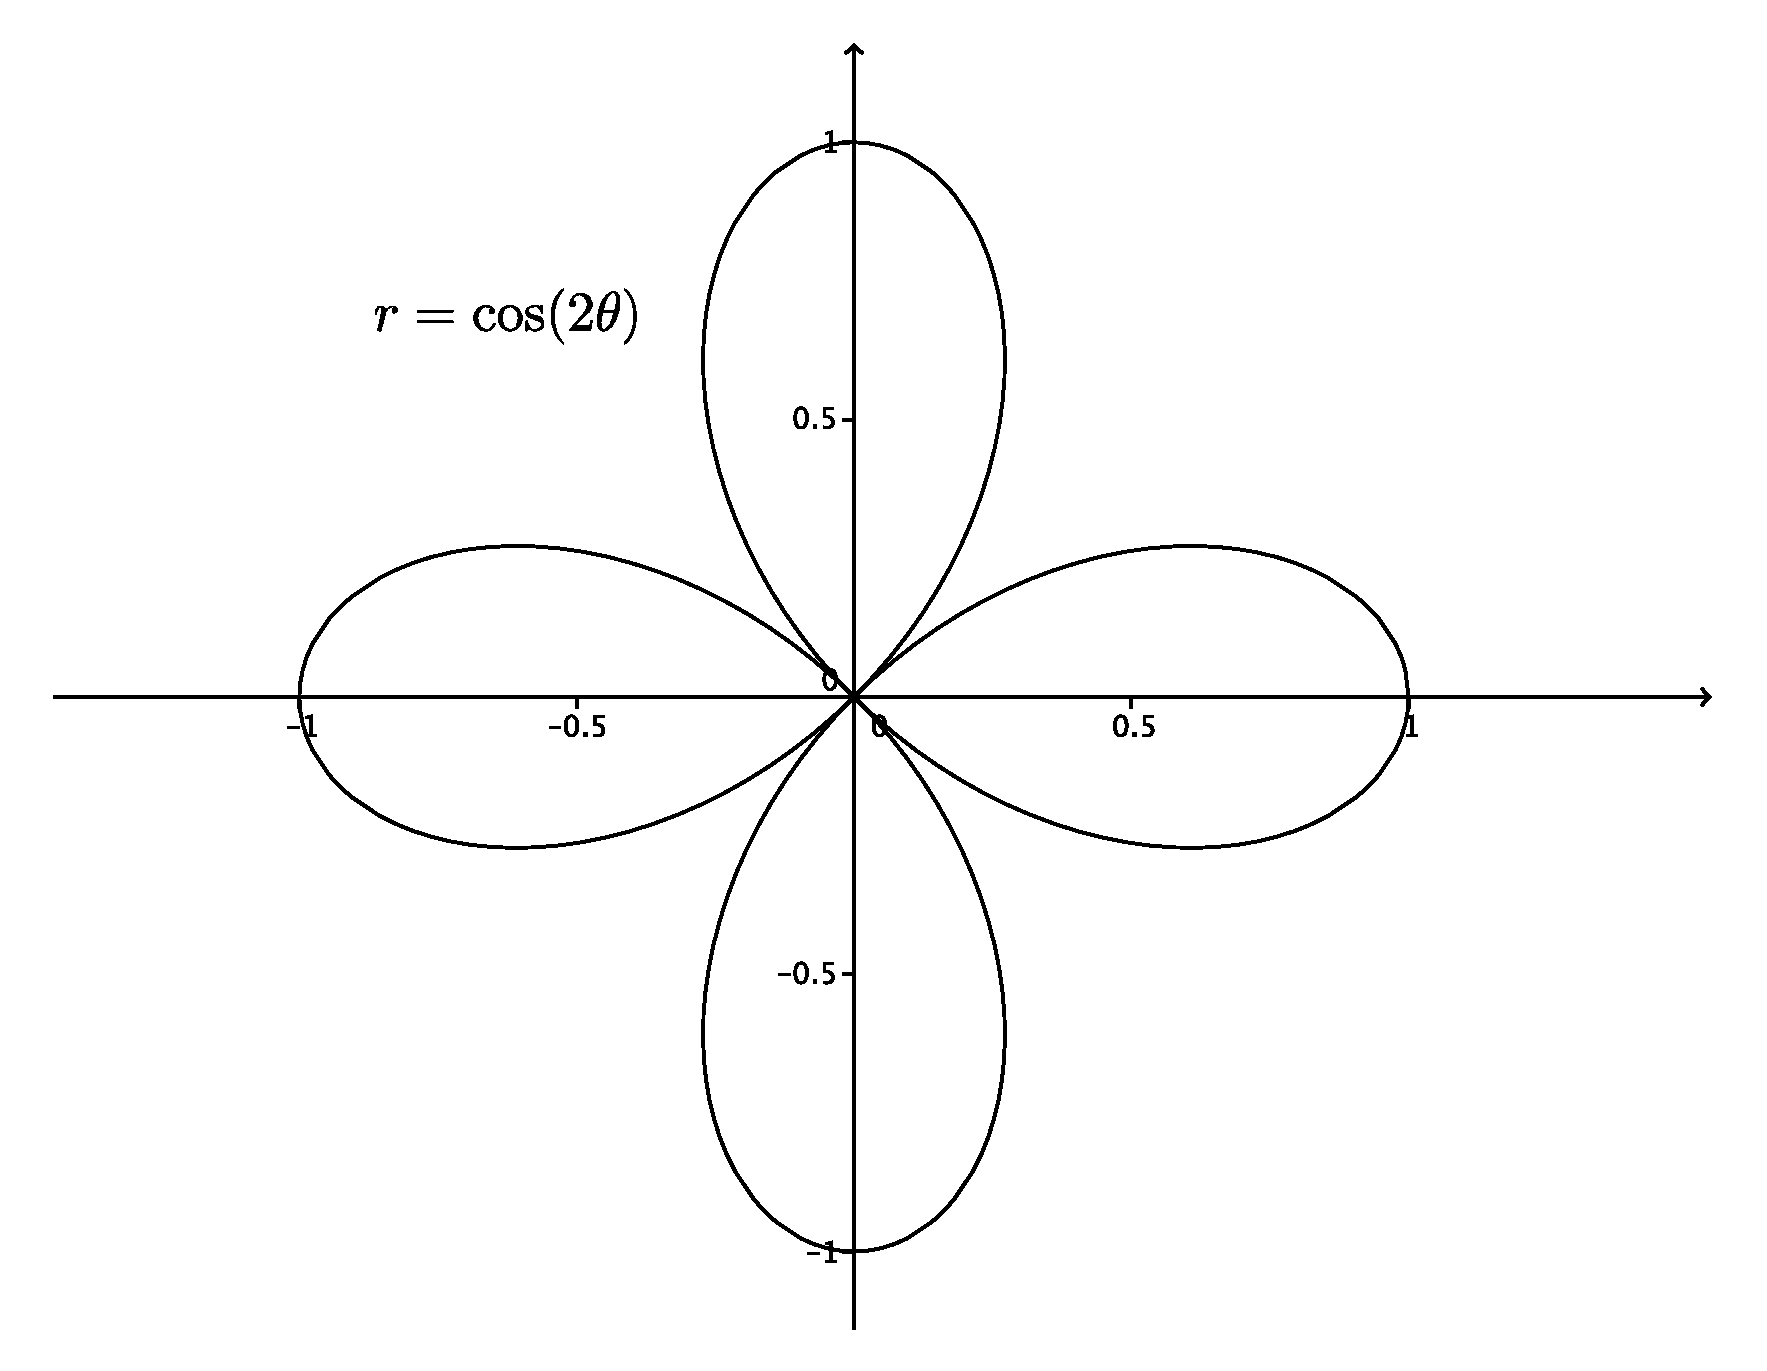
\includegraphics[width=0.5\textwidth]{WS6-1b}
\end{center}

Notice that we start with $r=1$ when $\theta=0$, then hit $r=0$ at $\pi/4$. For $\pi/4<\theta<3\pi/4$, $r$ is negative, so we trace the curve on the opposite side of the origin, hitting $r=-1$ at $\theta=\pi/2$, and so on.

\item $r=2\cos(\theta)$, $\theta\in [-\pi/2,\pi/2]$

\begin{center}
 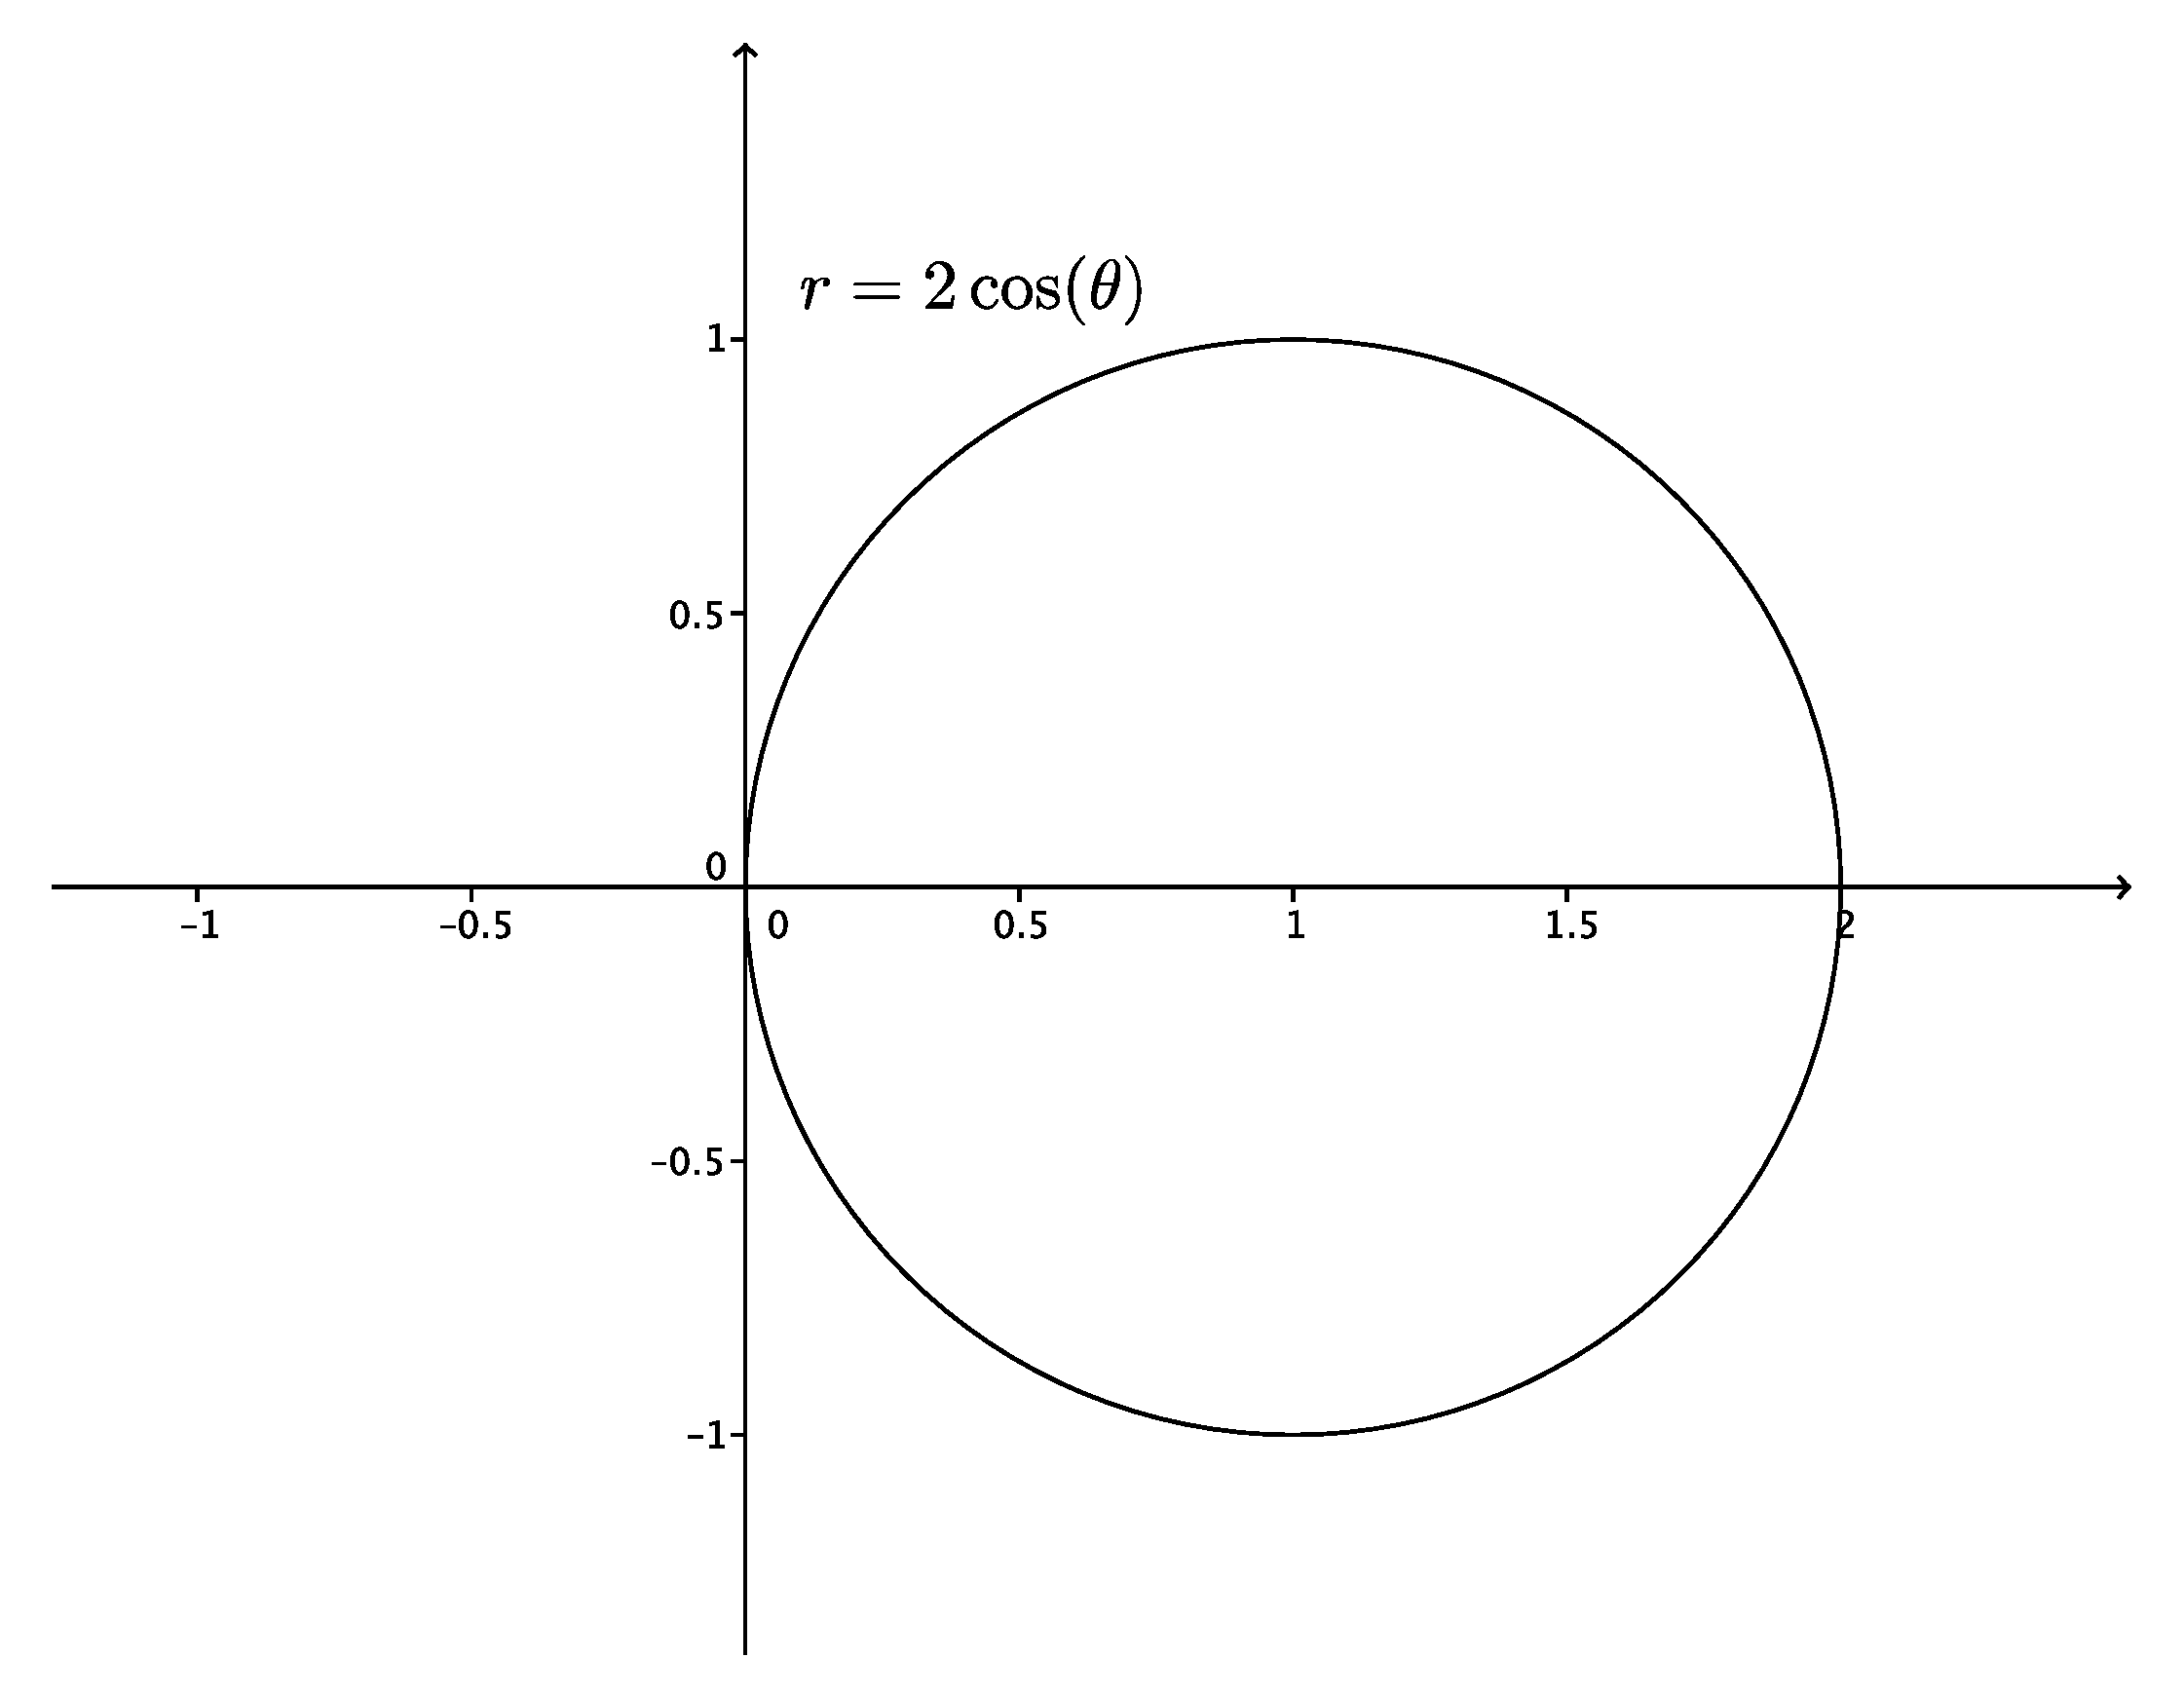
\includegraphics[width=0.5\textwidth]{WS6-1c}
\end{center}

Note that this is indeed a circle: if $r=2\cos\theta$, then $r^2=2r\cos\theta$, so $x^2+y^2=2x$. Completing the square gives $(x-1)^2+y^2=1$.
\end{enumerate}
\newpage

\item Find the given area:
\begin{enumerate}
\item Inside the circle $r=2\cos\theta$, but outside the circle $r=2\sin\theta$.

\begin{center}
 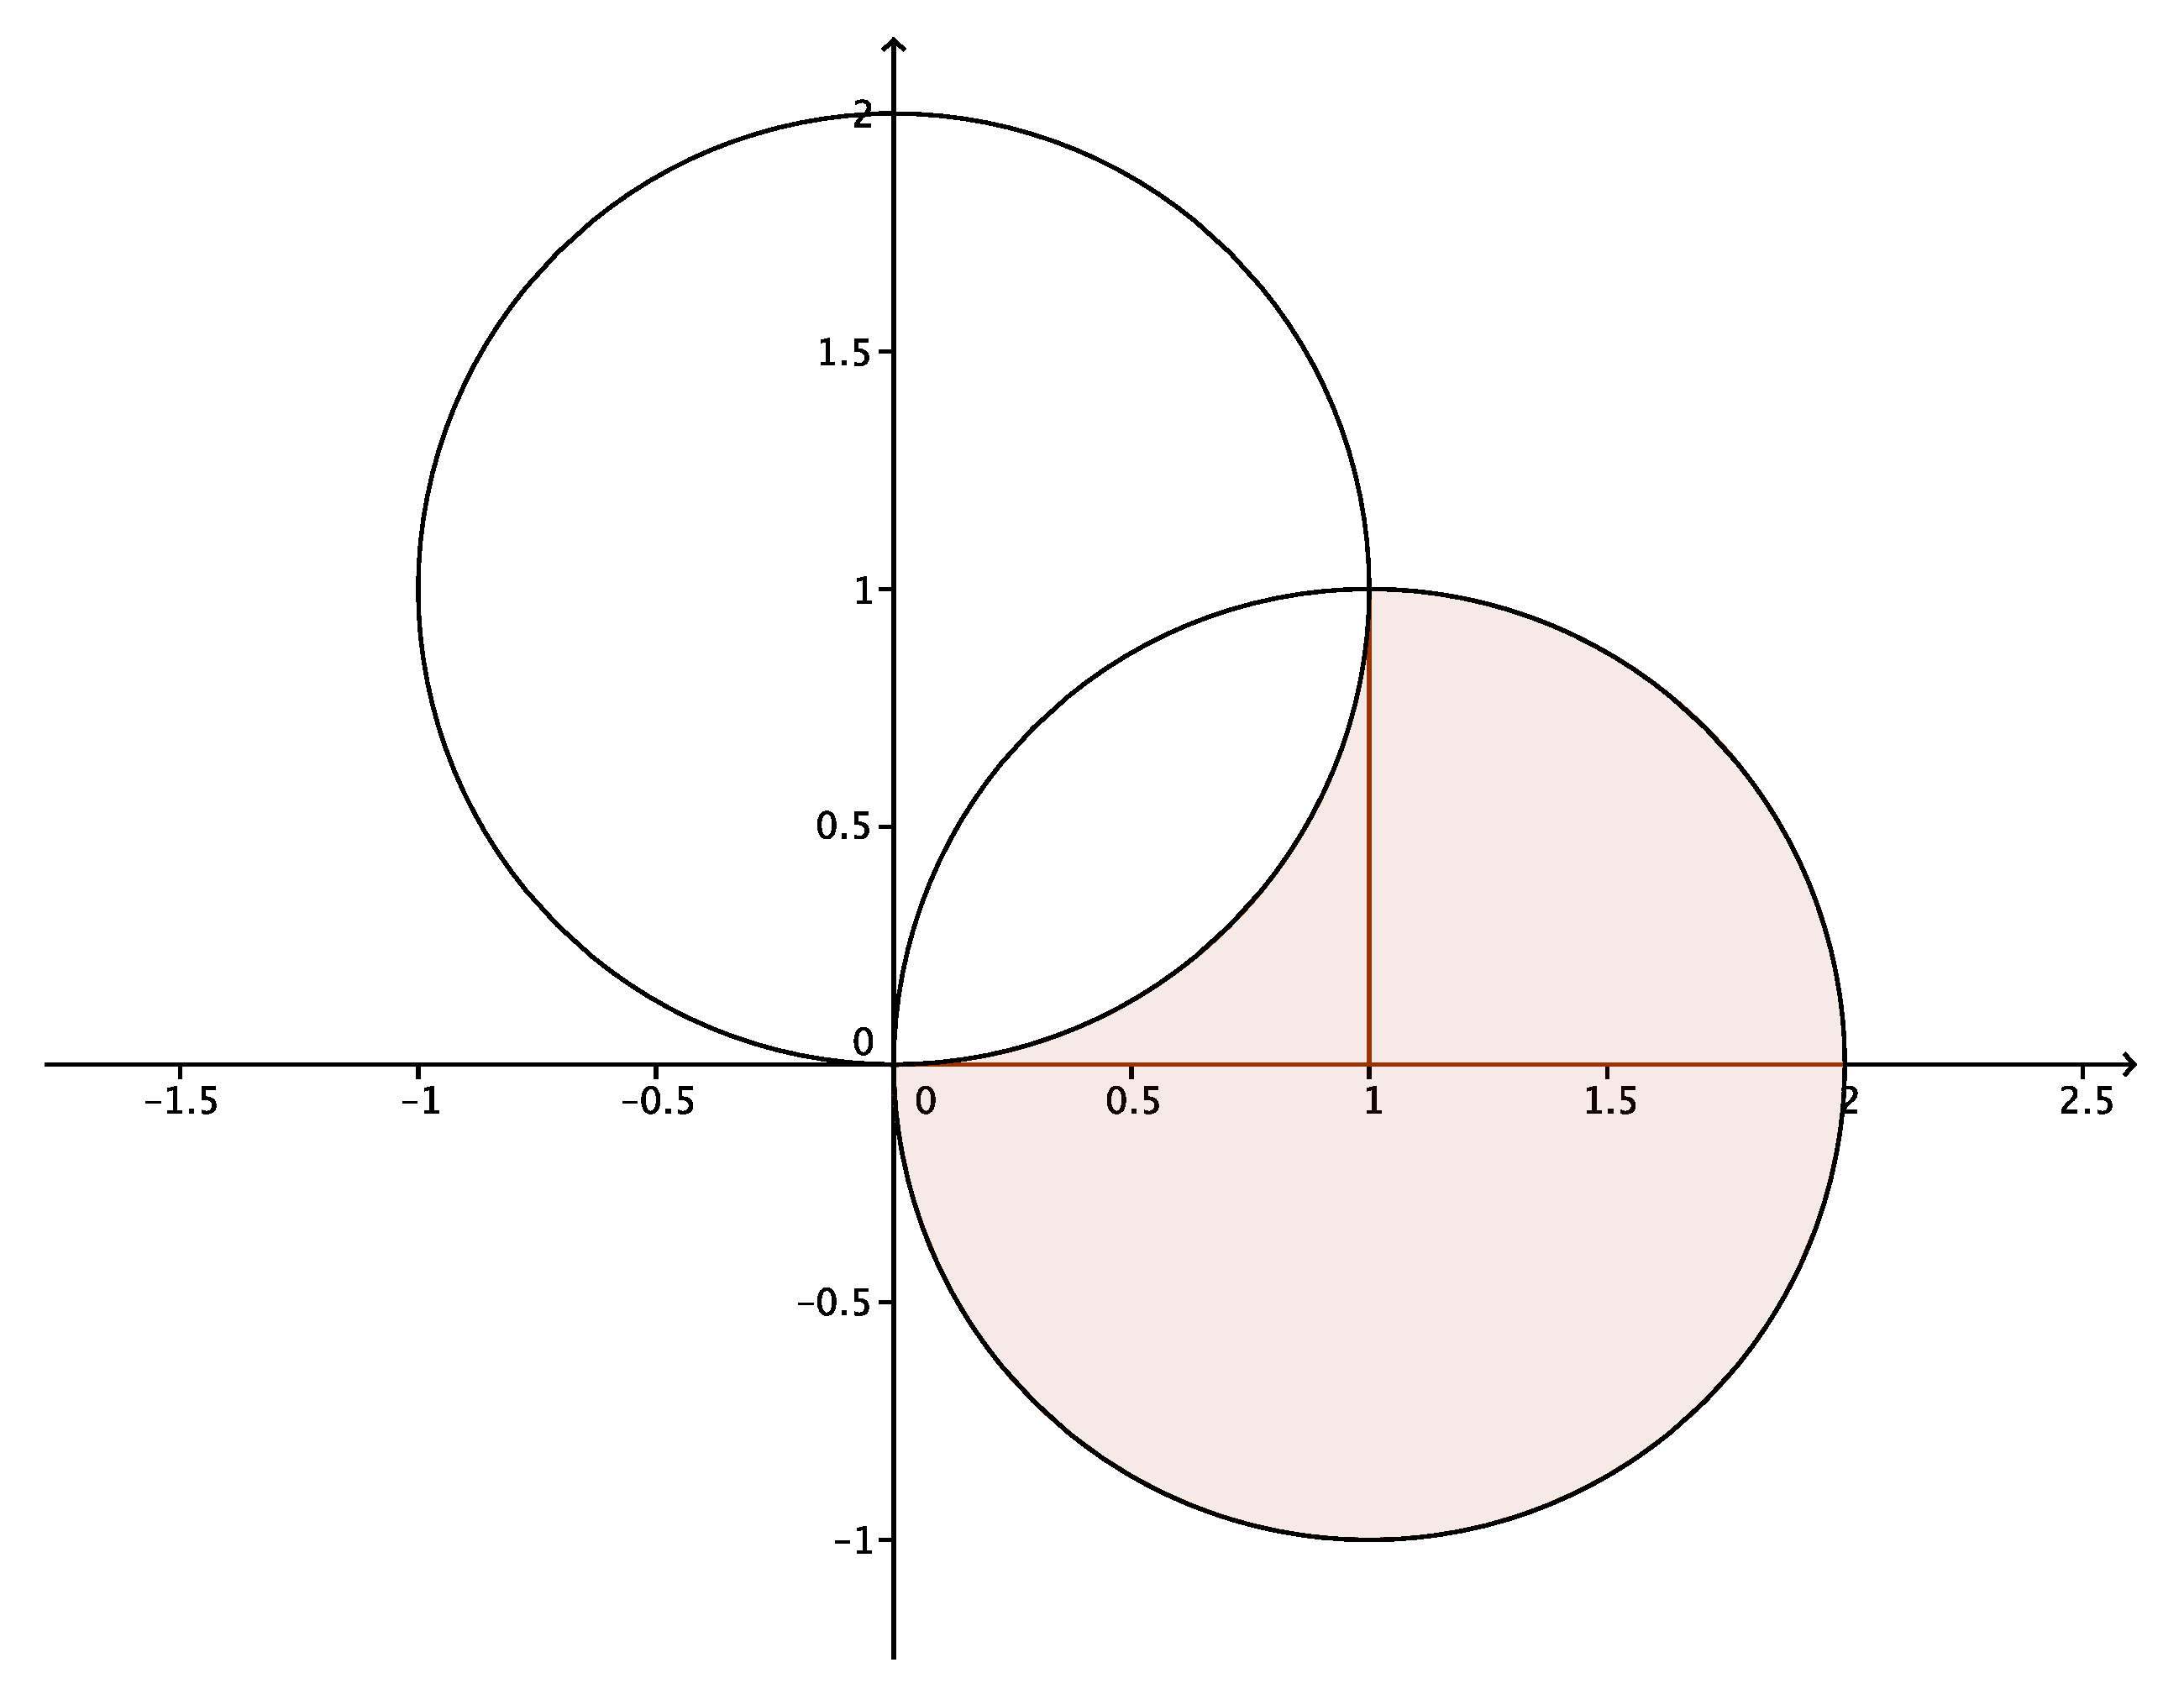
\includegraphics[width=0.6\textwidth]{WS6-4c}
\end{center}

The desired area consists of two parts: the half of the circle $r=2\cos\theta$ that lies below the $x$-axis, which has area $\pi/2$, and the part of this circle above the $x$-axis that is outside the circle $r=2\sin\theta$. Noting that the two circles intersect when $\theta=\pi/4$, this area can be computed by finding the area inside the circle $r=2\cos\theta$ for $0\leq \theta\leq \pi/4$, and subtracting the area that lies inside the circle $r=2\sin\theta$ on this same interval. Thus,
\begin{align*}
 A & = \frac{\pi}{2} + \frac{1}{2}\int_0^{\pi/4}((2\cos\theta)^2-(2\sin\theta)^2)\,d\theta\\
& = \frac{\pi}{2} + 2\int_0^{\pi/4}(\cos^2\theta-\sin^2\theta)\,d\theta\\
& = \frac{\pi}{2} + 2\int_0^{\pi/4}\cos(2\theta)\,d\theta\\
& = \frac{\pi}{2} + \sin(2\theta)\vert_0^{\pi/4} = \frac{\pi}{2}+1.
\end{align*}
\newpage

\item The area common to the inside of the curves $r=\cos\theta$ and $r=\sin(2\theta)$, in the first quadrant.

\begin{center}
 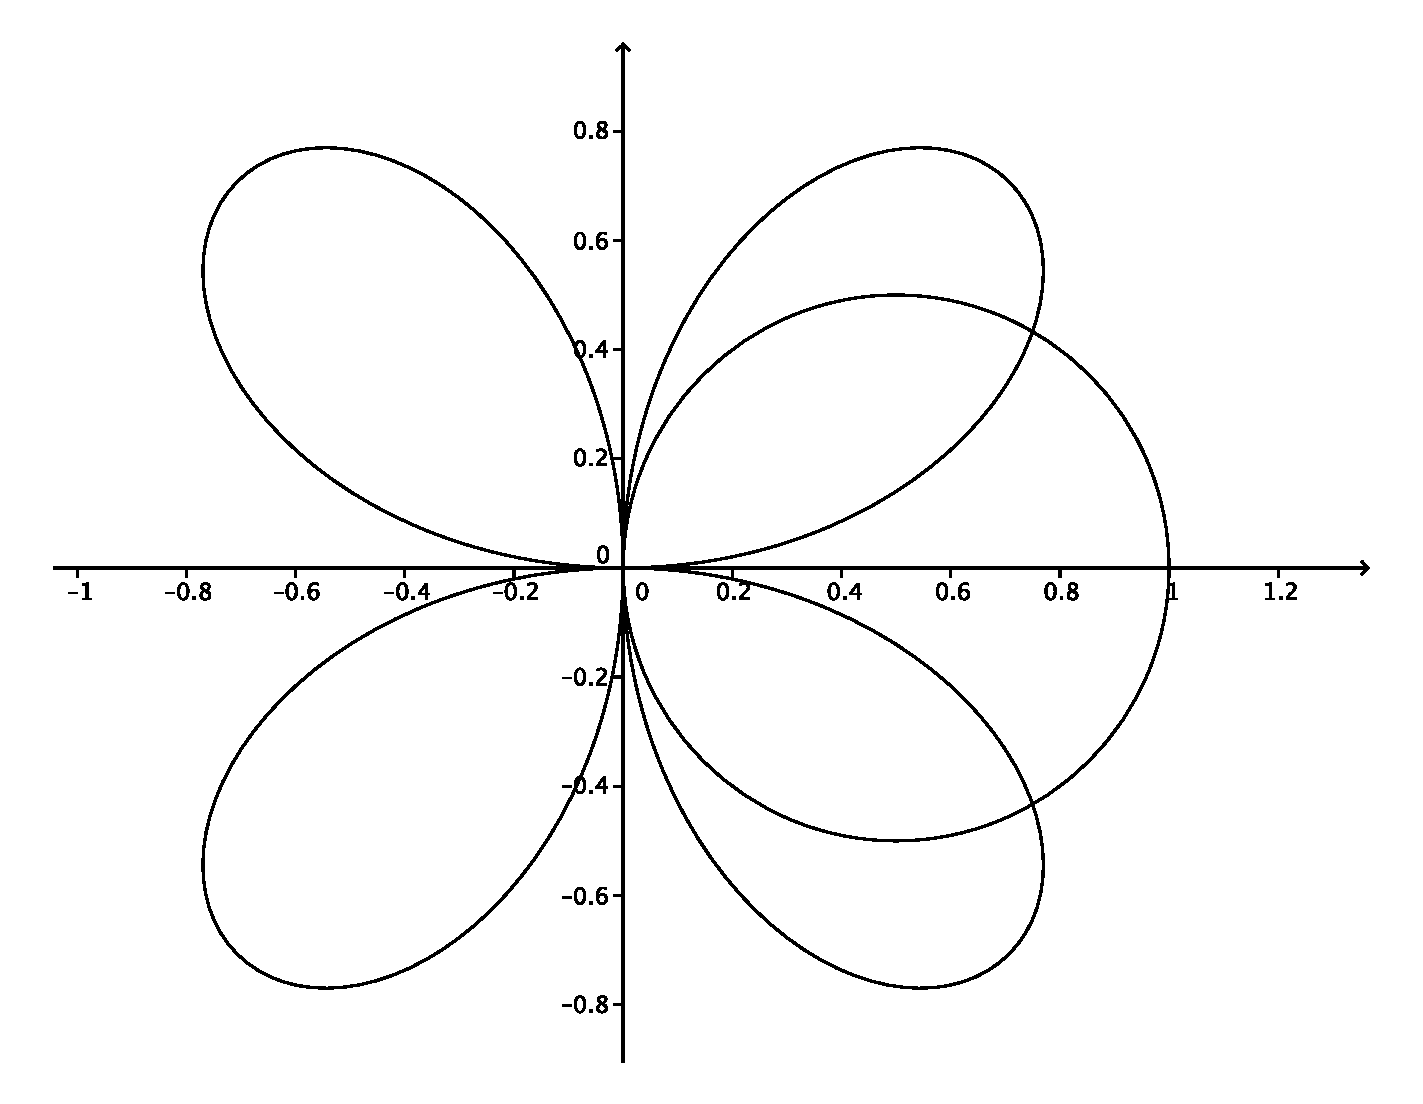
\includegraphics[width=0.6\textwidth]{WS6-4d}
\end{center}

The point of intersection between the two curves in the first quadrant occurs when $\theta = \pi/6$. From the diagram, we can see that the area common to the inside of the two curves can be described as follows:

For $0\leq \theta\leq \dfrac{\pi}{6}$, we have $0\leq r\leq \sin(2\theta)$.

For $\dfrac{\pi}{6}\leq \theta \leq \dfrac{\pi}{2}$, we have $0\leq r\leq \cos\theta$.

Thus, the area is given by
\begin{align*}
 A & = \frac{1}{2}\int_0^{\pi/6}\sin^2(2\theta)\,d\theta + \frac{1}{2}\int_{\pi/6}^{\pi/2}\cos^2\theta\,d\theta\\
& = \frac{1}{4}\int_0^{\pi/6}(1-\cos(4\theta))\,d\theta + \frac{1}{4}\int_{\pi/6}^{\pi/2}(1+\cos(2\theta))\,d\theta\\
& = \frac{\pi}{8}-\frac{3\sqrt{3}}{32}.
\end{align*}

\end{enumerate}
\newpage

\item Show that the indicated limit does not exist:
\begin{enumerate}
\item $\di\lim_{(x,y)\to (0,0)}\frac{3x+4y}{x-2y}$

If we approach the origin along the $x$-axis, we have $y=0$ and we get 
\[
\lim_{x\to 0}\frac{3x}{x}=3.
\]
If we approach the origin along the $y$-axis, we have $x=0$, and we get
\[
\lim_{y\to 0}\frac{4y}{-2y}=-2.
\]
Since we get different limits along different paths, the limit must be zero.

\item $\di\lim_{(x,y)\to (0,0)}\frac{xy^4}{x^2+y^8}$

If we approach the origin along either axis, the limit is clearly zero. (Indeed, the limit is zero along any straight line $y=kx$ through the origin!)

However, if we approach the origin along the curve $x=y^4$, we get
\[
\lim_{y\to 0}\frac{y^4\cdot y^4}{(y^4)^2+y^8}=\lim_{y\to 0}\frac{y^8}{2y^8} = \frac12.
\]
Since we get different limits along different paths, the limit does not exist.

\end{enumerate}

\item What geometric object is obtained as the graph of $f(x,y)=2x-3y$?

The graph $z=f(x,y)$ gives us the equation $z=2x-3y$, or $2x-3y-z=0$. This is a plane through the origin with normal vector $\vec{n}=\langle 2,-3,-1\rangle$.

\item \textit{Challenge:} Describe the level surfaces of $f(x,y,z)=k$ $f(x,y,z)=x^2+y^2-z^2$, for $k=-2,-1,0,1,2$.

For $k=1, 2$, (or any $k>0$) the equation $x^2+y^2-z^2=k$ is a hyperboloid of one sheet. For $k=-1,-2$, the equation $x^2+y^2-z^2=k$ is a hyperboloid of two sheets. For $k=0$, we get $x^2+y^2=z^2$, which is a cone.

To explore this with computer-aided graphics, see \href{https://www.geogebra.org/m/QtWZfC3Z}{https://www.geogebra.org/m/QtWZfC3Z}
\end{enumerate}

\newpage


Extra practice:
\begin{enumerate}
\item Plot the polar function:
\begin{enumerate}
\item $r=2+\cos\theta$, $\theta\in [0,2\pi]$

\begin{center}
 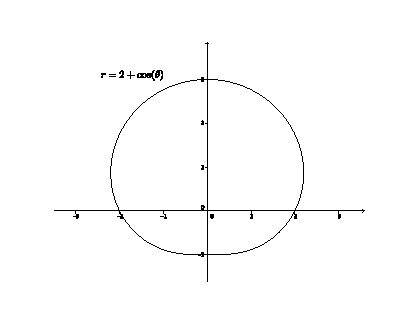
\includegraphics[width=0.6\textwidth]{WS6-1a}
\end{center}

\item $r^2=\cos(2\theta)$, $\theta\in [-\pi/4,\pi/4]\cup [3\pi/4,5\pi/4]$

\begin{center}
 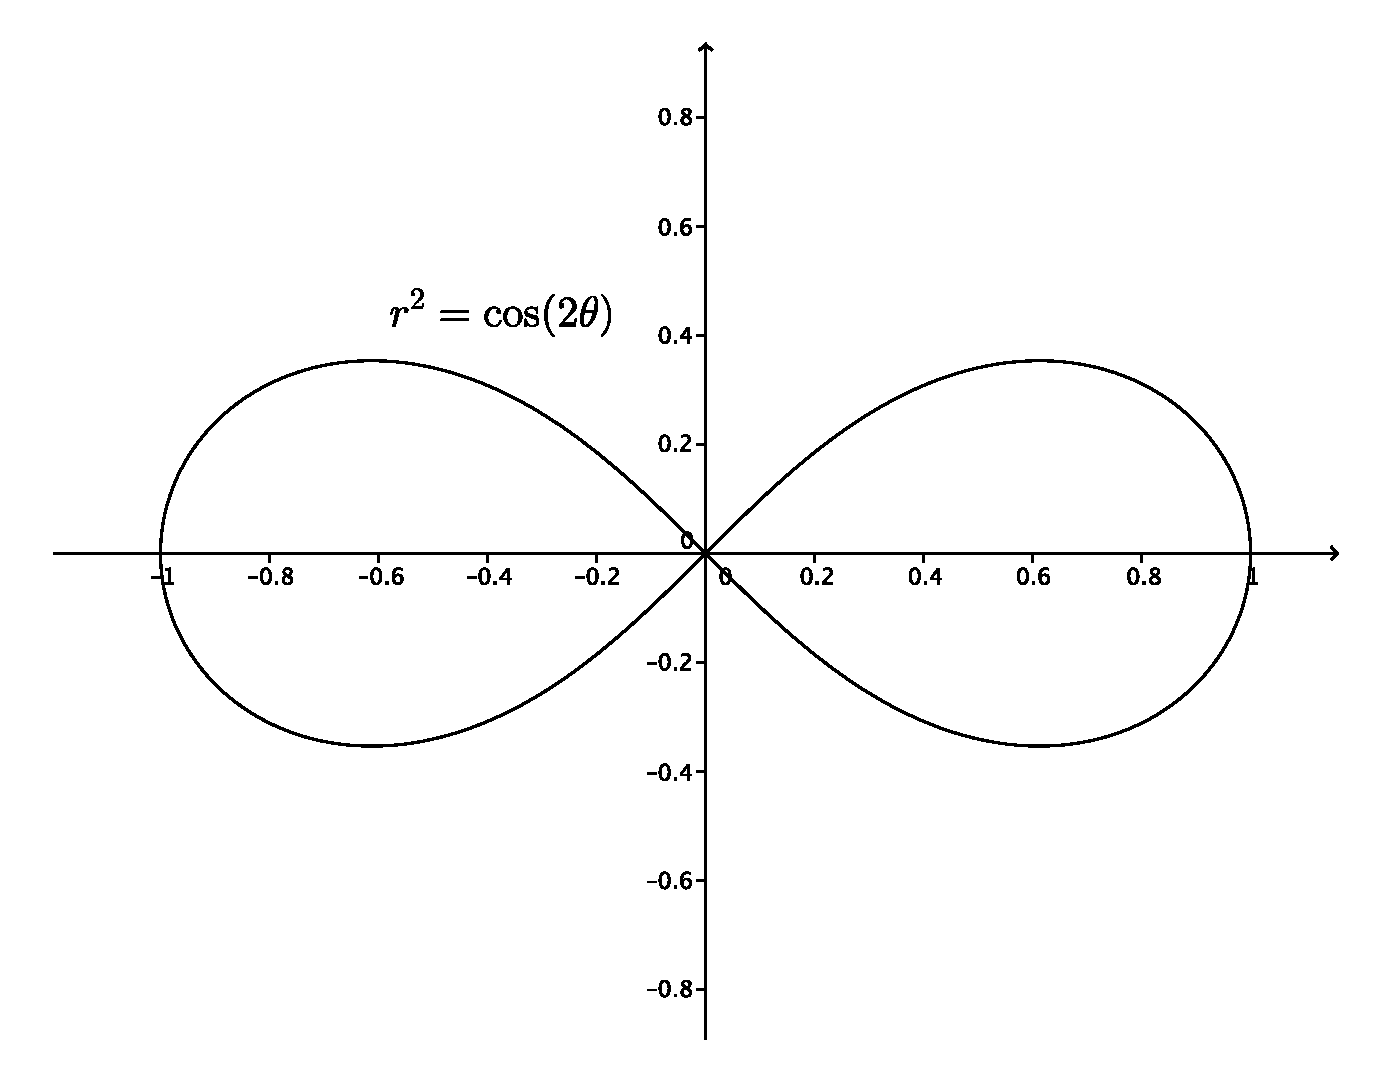
\includegraphics[width=0.6\textwidth]{WS6-1d}
\end{center}
\end{enumerate}

\newpage

\item Find the points of intersection of the polar curves. (Note that the point $(0,0)$ requires special care: you might have $r=0$ for \textit{different} values of $\theta$ for the two curves.)
\begin{enumerate}
\item $r=\cos(2\theta)$ and $r=\cos\theta$, on $[0,2\pi]$

To help us be sure we've found all the points of intersection, we plot the two curves:

\begin{center}
 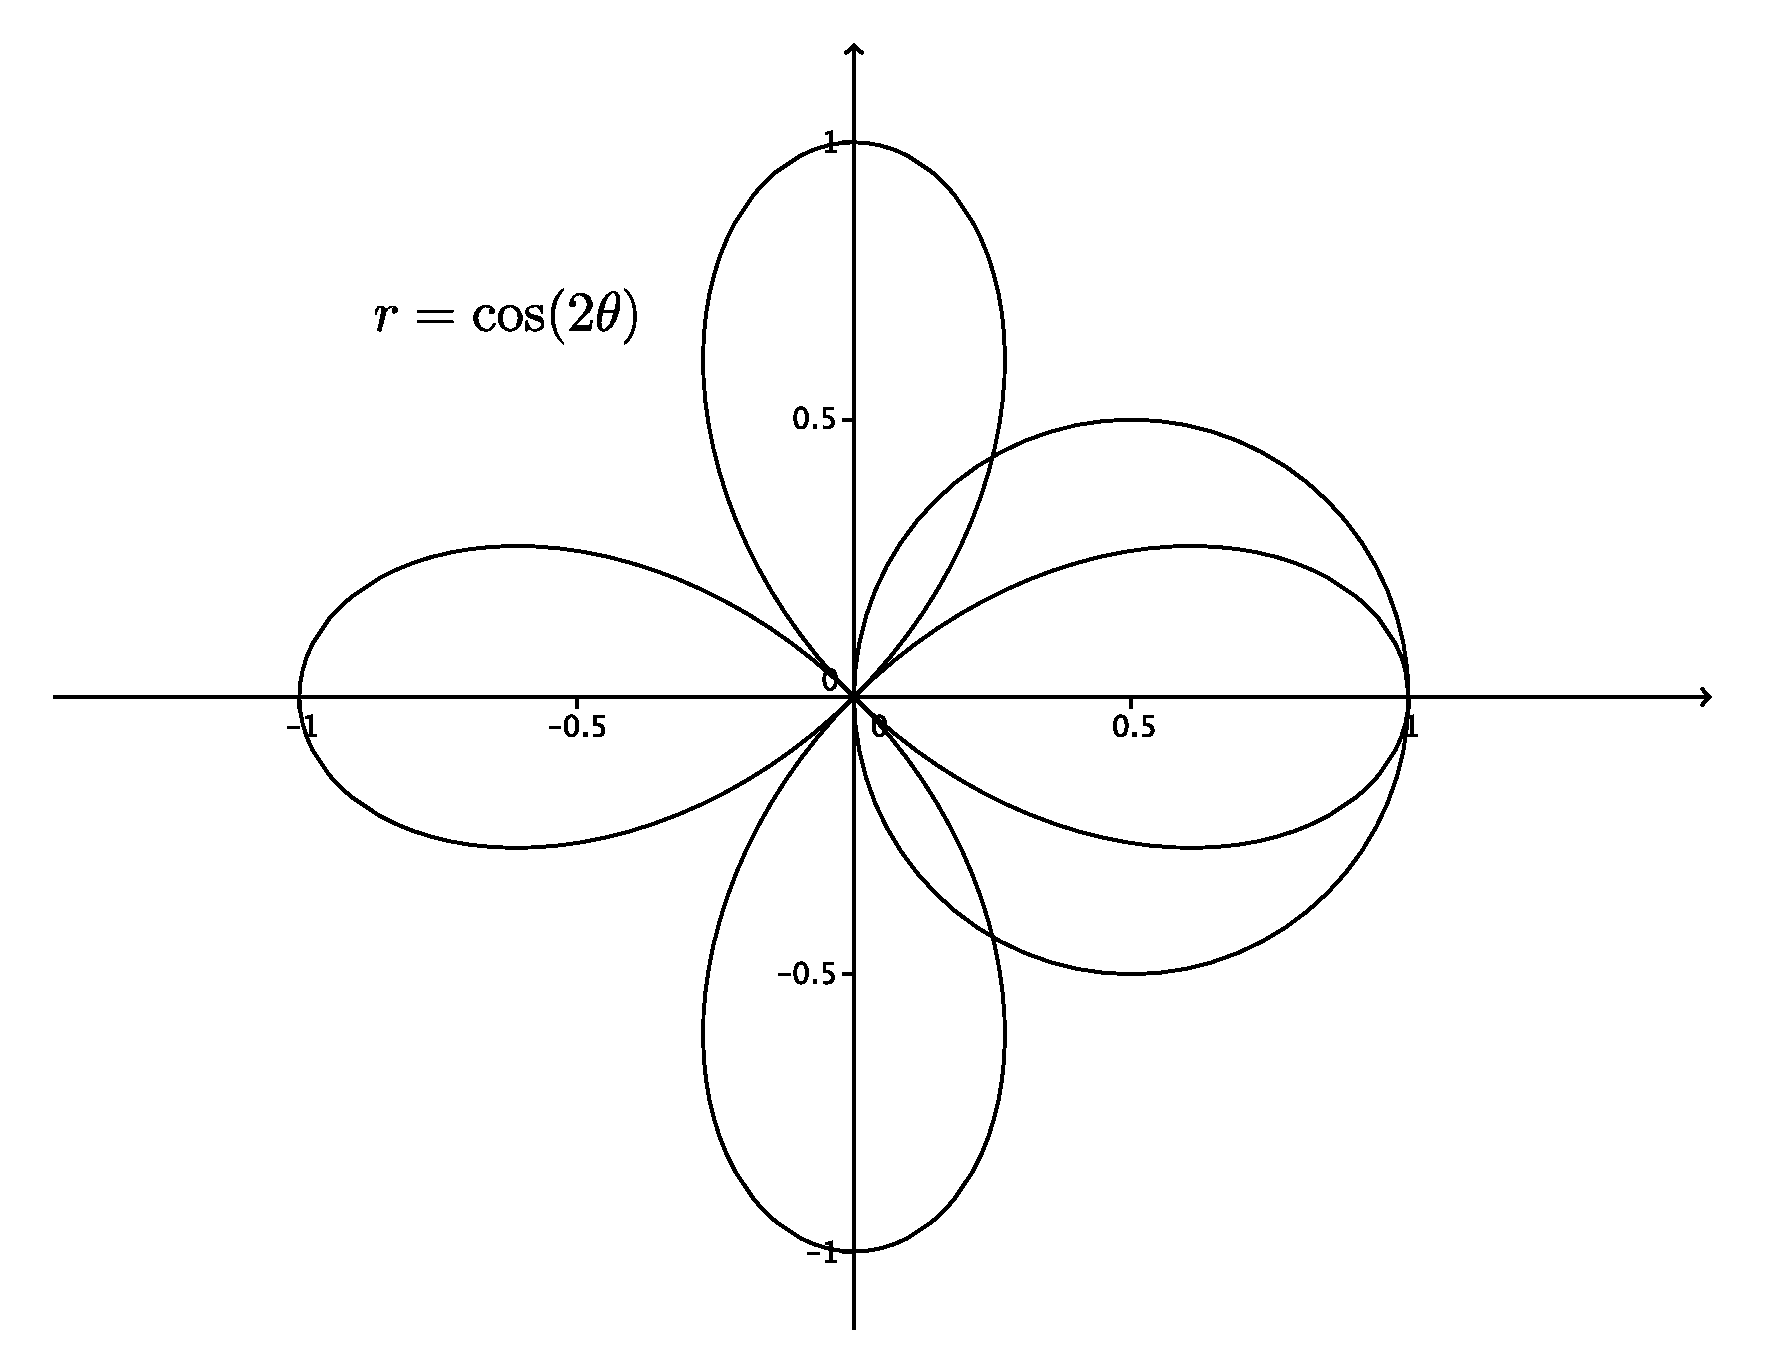
\includegraphics[width=0.6\textwidth]{WS6-3a}
\end{center}

From the plot, we see that there should be four points of intersection, and one of the points is the origin. The origin is given by $r=0$, for \textbf{any} value of $\theta$. (This is the one drawback of polar coordinates: we have one point that does not determine a unique set of values for $r$ and $\theta$. (OK, technically this is true of all points, since we can always add $2\pi$ to $\theta$, but we can always restrict the interval for $\theta$.))

For the curve $r=\cos(2\theta)$, $r=0$ gives $\cos(2\theta)=0$, so $2\theta$ must be an odd multiple of $\pi/2$. On the interval $[0,2\pi]$, this happens for $\theta = \pi/4, 3\pi/4, 5\pi/4$, and $7\pi/4$. On the other hand, setting $r=0$ in the equation $r=\cos\theta$ gives us $\theta = \pi/2$ or $\theta = 3\pi/2$. Even though none of the $\theta$ values agree, $(0,0)$ is nonetheless a point of intersection.

Now, for the other points of intersection, $r\neq 0$, so we must have $\cos(2\theta)=\cos(\theta)$. Since $\cos(2\theta) = 2\cos^2\theta-1$, we get $2\cos^2(\theta)-1=\cos(theta)$, or $2\cos^2\theta-\cos(\theta)-1 = (2\cos(\theta)+1)(\cos\theta-1)=0$. Thus, either $\cos\theta = -\dfrac{1}{2}$, giving us either $\theta = 2\pi/3$ or $\theta = 4\pi/3$, or $\cos\theta = 1$, giving us $\theta=0$ or $\theta = 2\pi$.

Using the curve $r=\cos(\theta)$, we have $x=\cos^2\theta$ and $y=\cos\theta\sin\theta$. When $\theta = 2\pi/3$, we have $x=\left(\frac{-1}{2}\right)^2 = \frac{1}{4}$ and $y = -\frac{1}{2}\cdot \frac{\sqrt{3}{2}} = -\frac{\sqrt{3}}{4}$, so this is the point of intersection below the $y$-axis seen above. Similarly, when $\theta = 4\pi/3$, we get $x=\frac{1}{4}$ and $y = \frac{\sqrt{3}}{4}$, so this is the point of intersection above the $y$-axis. Finally, putting $\theta=0$ (or $2\pi$) gives us the point of intersection $(1,0)$.

\newpage

\item $r=\sin\theta$ and $r=\sqrt{3}+3\sin\theta$, on $[0,2\pi]$

From the plot below, we see that there are three points of intersection: one at the origin, and one in each of the first and second quadrants.


\begin{center}
 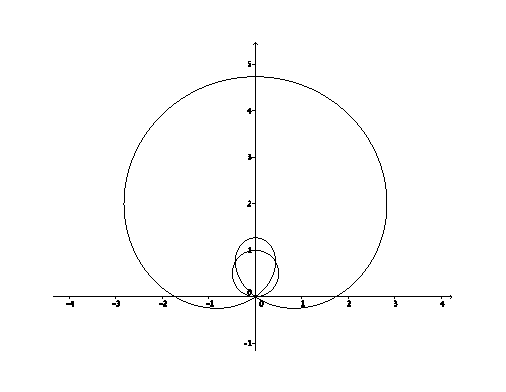
\includegraphics[width=0.6\textwidth]{WS6-3b}
\end{center}

As above, we confirm the intersection at the origin as a special case. The first curve passes through the origin for $\theta = 0, \pi, 2\pi$, and the other when $\sin(\theta) = -\dfrac{1}{\sqrt{3}}$. For the other two points of intersection, we set $\sin\theta = \sqrt{3}+3\sin\theta$, giving us $\sin\theta = -\dfrac{\sqrt{3}}{2}$, so $\theta = 4\pi/3$ or $\theta = 5\pi/3$. Using $r=\sin\theta$, we have $x = \sin\theta\cos\theta$ and $y=\sin^2\theta$. When $\theta = 4\pi/3$, we have $x=(-\sqrt{3}/2)(-1/2) = \sqrt{3}/4$, while $y = (\sqrt{3}/2)^2 = 3/4$. Thus, the point of intersection in the first quadrant is $\left(\frac{\sqrt{3}{4}},\frac{3}{4}\right)$. Similarly, we find that the point of intersection in the second quadrant is $\left(\frac{-\sqrt{3}}{4},\frac{3}{4}\right)$.

\end{enumerate}
\newpage

\item Compute the area:
\begin{enumerate}
\item One loop of the three-leaf rose $r=\sin(3\theta)$.

\begin{center}
 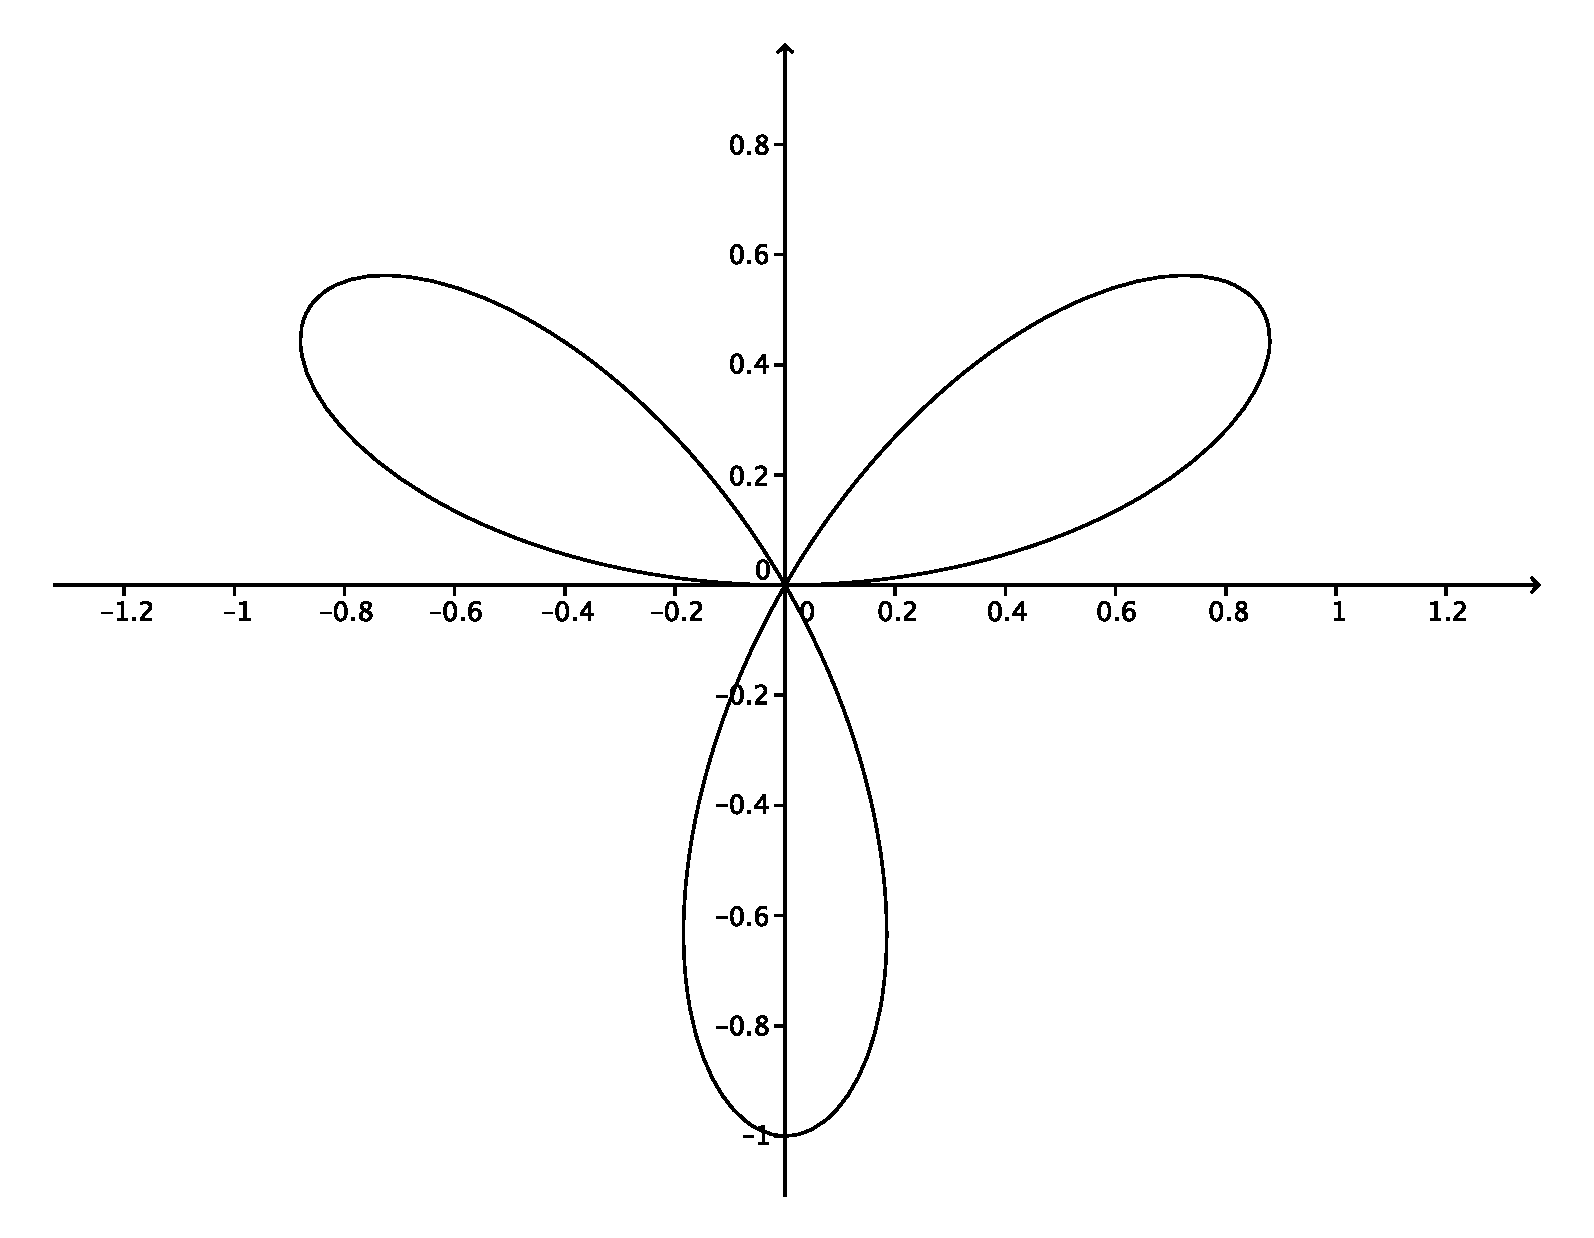
\includegraphics[width=0.6\textwidth]{WS6-4a}
\end{center} 

The three-leaf rose is pictured above. We'll find the area enclosed by the loop in the first quadrant. We note that $\sin(3(0))=0$, so the curve begins at the origin when $\theta=0$. As $\theta$ increases, we enter the first quadrant, and remain there until we reach $\sin(3\theta)=0$ again, which happens when $3\theta = \pi$, so $\theta = \pi/3$. Using the formula $\di A = \int_\alpha^\beta \frac{1}{2}r(\theta)^2\,d\theta$ for area, we thus have
\[
 A = \frac{1}{2}\int_0^{\pi/3}\sin^2(3\theta)\,d\theta = \frac{1}{4}\int_0^\pi/3 (1-\cos(6\theta))\,d\theta = \frac{1}{4}(\frac{\pi}{3}) = \frac{\pi}{12}.
\]
\newpage
\item The outer loop of the lima{\c c}on $r=1+2\cos\theta$.

\begin{center}
 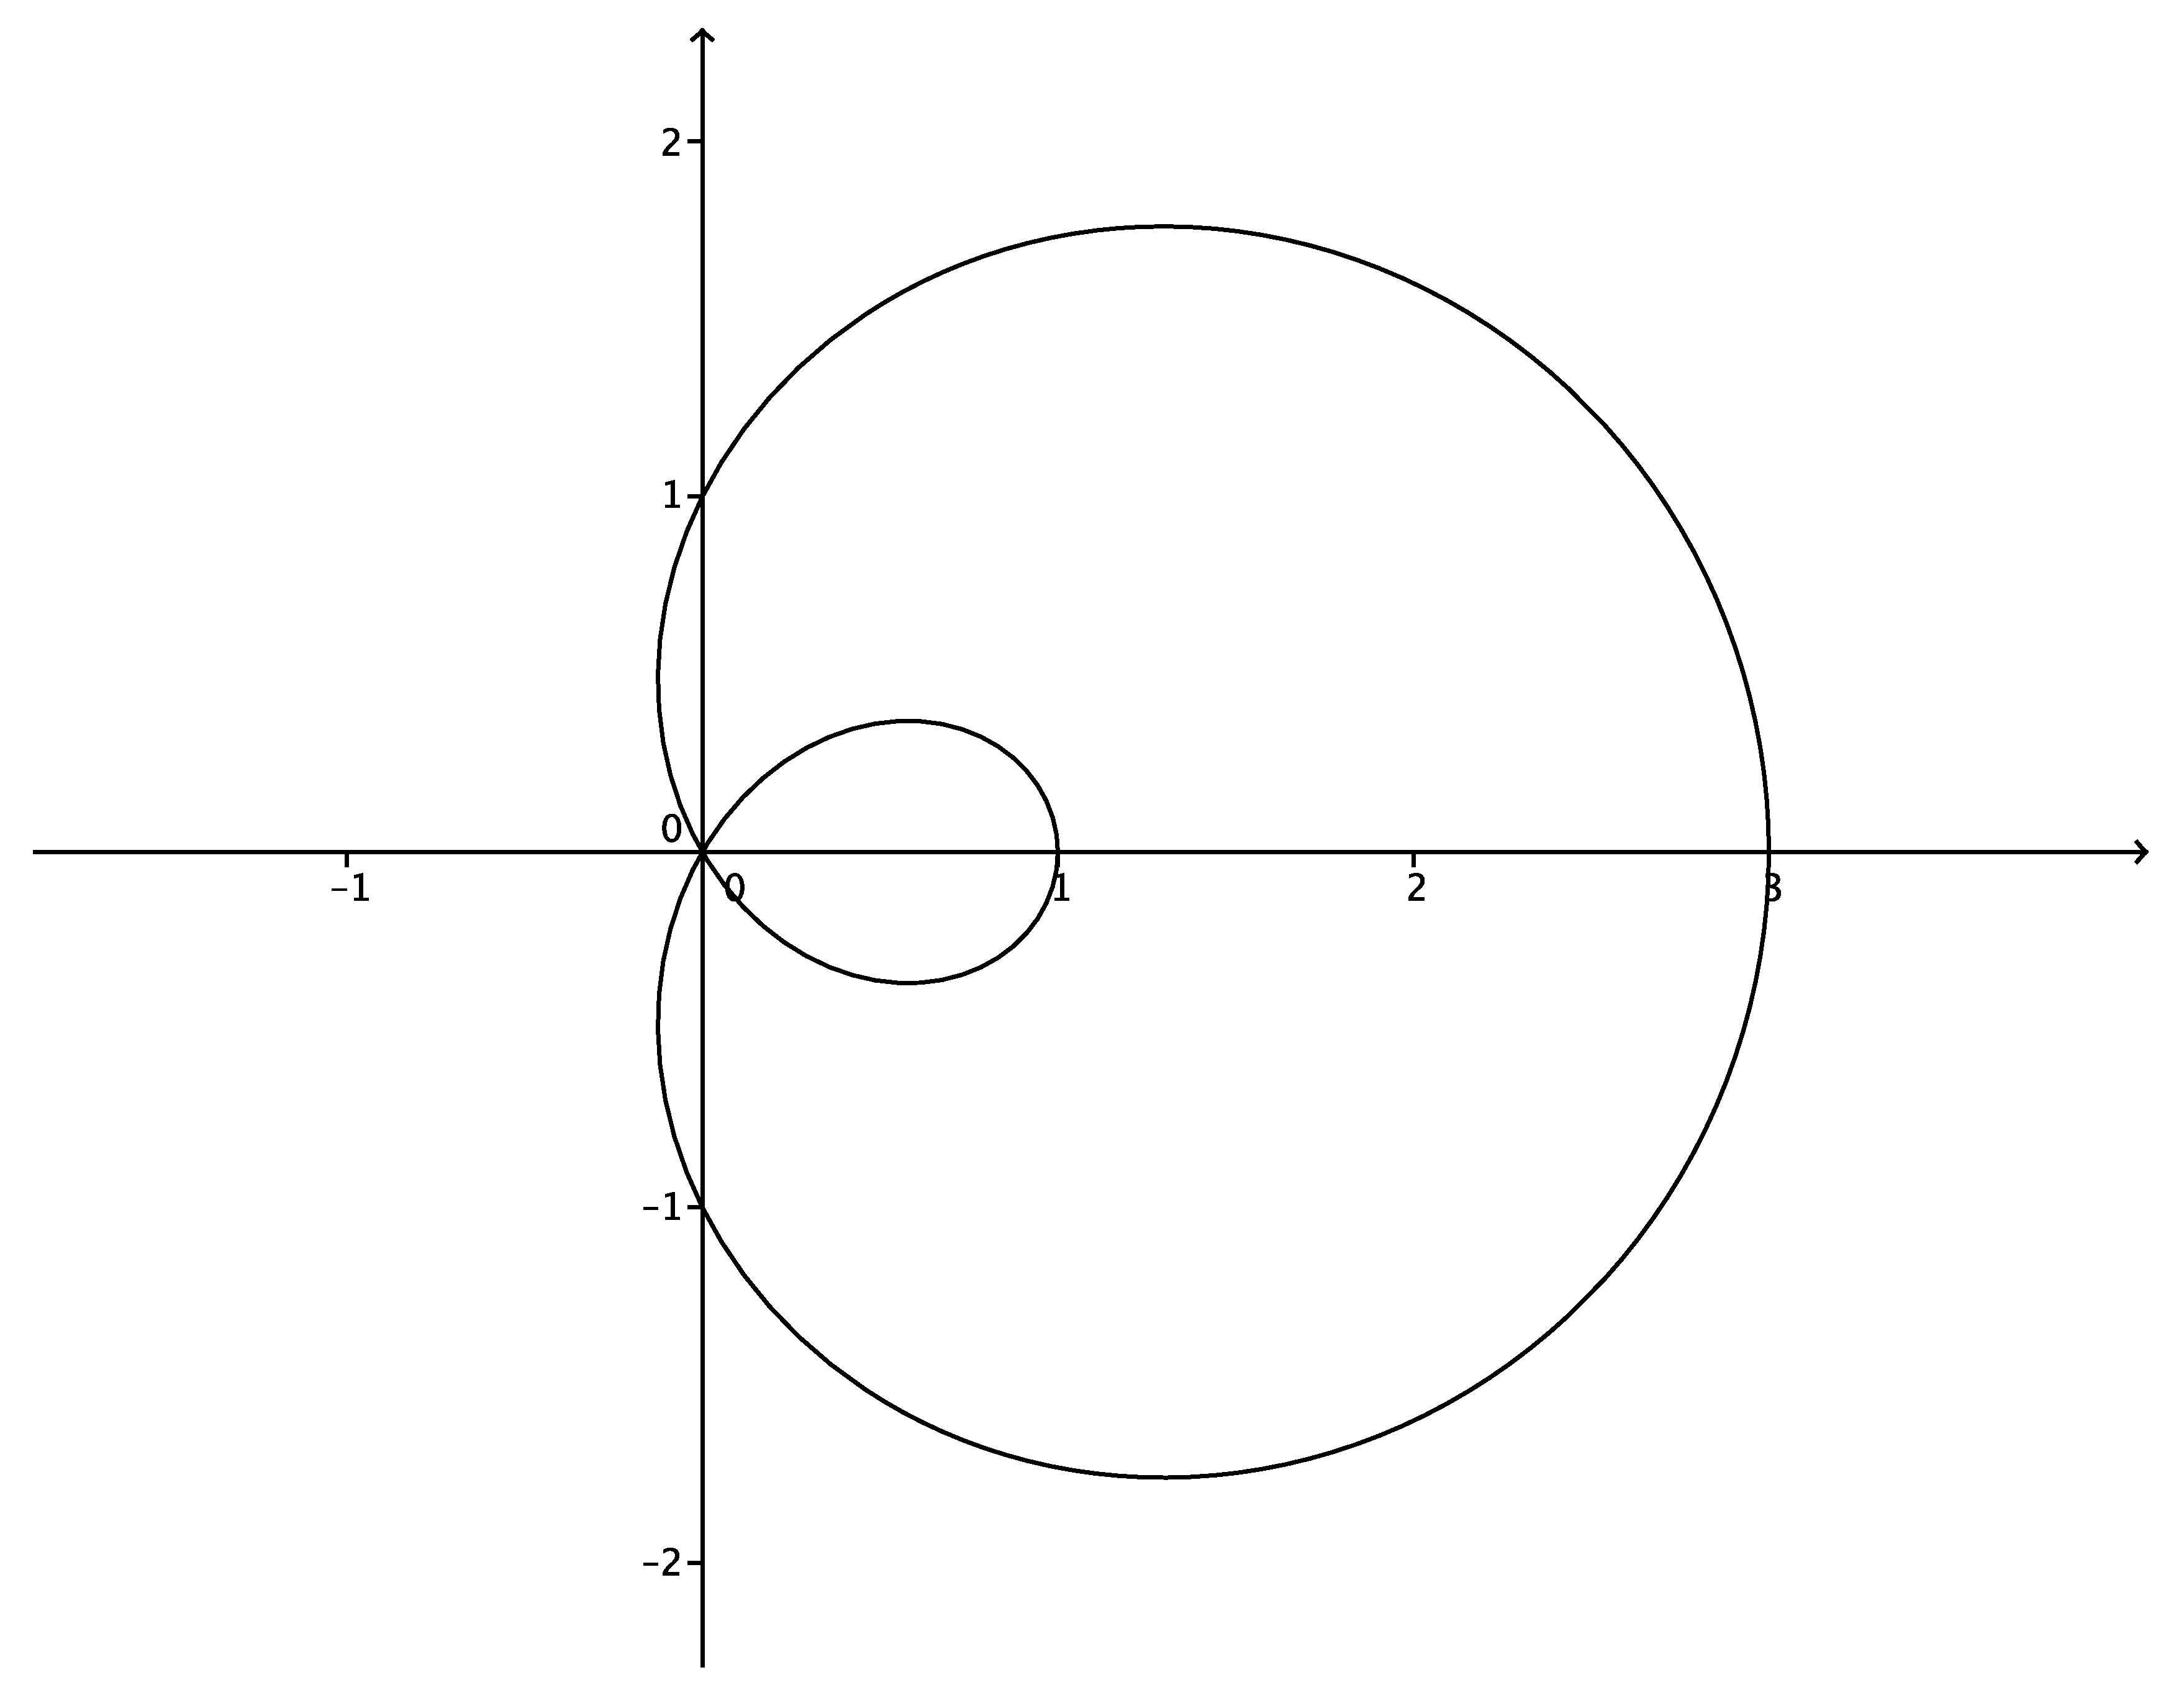
\includegraphics[width=0.6\textwidth]{WS6-4b}
\end{center}

There's a bit of interpretation required here: does ``enclosed by the outer loop'' mean everything inside the outer loop, or does it mean everything that is inside the outer loop, but outside the inner loop? It seems more likely that it means the former. If we start at $\theta = 0$, we begin at $(3,0)$ and trace out the top half of the loop, returning to the origin when $\cos\theta = -1/2$, or $\theta = 2\pi/3$. For $2\pi/3\leq \theta\leq 4\pi/3$ we trace out the inner loop, and from $4\pi/3$ to $2\pi$ we get the bottom of the outer loop. By symmetry, the desired area is twice the area between the upper half of the outer loop and the $x$-axis. Thus,
\begin{align*}
 A &= 2\int_0^{2\pi/3}\frac{1}{2}(1+2\cos\theta)^2\,d\theta = \int_0^{2\pi/3}(1+4\cos\theta+4\cos^2\theta)\,d\theta\\
& = \int_0^{2\pi/3}(3+4\cos\theta+2\cos(2\theta)\,d\theta = \left. 3\theta+4\sin\theta+\sin(2\theta)\right|_0^{2\pi/3}\\
& = 2\pi+\frac{3\sqrt{3}}{2}
\end{align*}

Note: if you don't invoke symmetry, it's a good idea to replace the interval $[0,2\pi]$ with the interval $[-\pi,\pi]$. Leaving out the inner loop means integrating from $-2\pi/3$ to $2\pi/3$ rather than integrating from 0 to $2\pi/3$ and then from $4\pi/3$ to $2\pi$.

\end{enumerate}
\end{enumerate}

\end{document}